\documentclass[10pt,twocolumn]{article}

\usepackage{graphicx}
\usepackage[colorlinks=true,allcolors=blue]{hyperref}

\begin{document}

\title{Next-generation design tools for intelligent transportation systems}
\author{Dominik Ascher and Georg Hackenberg}
\maketitle

\begin{abstract}
    \textcolor{red}{TODO}
\end{abstract}

\section{Introduction}
\label{sec:introduction}

The transformative patterns of future mobility are enabled by interconnected and integrated systems and services.
As such, Intelligent Transportation Systems (ITS) establish new transportation paradigms such as connected and autonomous vehicles (CAV), multi-modal and demand-responsive transport systems, and facilitate the transportation electrification by efficient operation of electric vehicles. For this, complex scenarios and their encoded requirements need to be holistically addressed, from which integrated system designs have to be derived, which allow transport infrastructures and their heterogenous actors to be more efficient and sustainable.

Therefore, constituent systems need to be designed with respect to most efficient structures and control strategies within themselves, while accounting for and exploiting the emergent properties they achieve in conjunction and interdependence with other systems, as composed, integrated system-of-systems (SoS). To systematically support the aforementioned systems engineering task, model- and simulation-based systems engineering~\cite{gianni2014modeling} can be employed for abstraction of design problems through the use of system models and their evaluation, i.e. their numerical approximation in terms of concrete behavior at run time. For this, well-defined system models are formulated at design time, for which then simulation aids projecting run-time information and performance metrics about the system under design and its environment. 
However, as systems and their underlying requirements are typically imperfectly understood at the beginning of the design task, methods and tools are needed to explore the possible design space, which support evaluation of system design alternatives and verification of intended system properties. 

%As an effect of underspecified requirements, system models are often not completely understood, and modeling uncertainties need be adressed. 

%Both structural as well as behavioral system design tasks can be supported using an overarching system design methodology at design time as well as at run time. 
%In terms of benefits, on the one hand side, system models faciliate gaining improved system understanding through specification, while allowing rapid system modification through defined variation points for designing a system. On the other hand side, simulation aids approximating information about the system dynamics and performance of a system under design.

For this, in previous work, we established an integrated systems modeling technique for integrated transportation and power systems. Here, our systems modeling technique allows one to model both transportation and power system scenarios, as well as mobility-on-demand scenarios to assess system design options systematically and improving system understanding holistically, based on a formal foundation~\cite{ascher_hackenberg_2014,ascher_hackenberg_2015,ascher_hackenberg_2016,ascher_hackenberg_2017}. The formal foundation was extended by a discrete event formalism \cite{ascher2023discrete} as well as integration with state-of-the-art simulators and predictive models for control strategy optimization \cite{ascher_hackenberg_albayrak_2023}.

\paragraph{Research objective}

With our research, we want to help improve the efficiency and effectiveness of today's transportation systems.
To achieve this goal, we work on methodologies for designing such systems and verifying their properties.
Fundamentally, we promote a formal approach capturing the relevant design decisions and their relations.
Furthermore, we integrate scenario-based simulation of system dynamics and evaluation of emergent properties.
Finally, we exploit optimization algorithms for optimizing system dynamics as well as static design decisions.

\paragraph{Research question}

In this paper, we ask how the next generation of design tools for intelligent transportation systems should look like.
Therefore, first we want to understand which system properties and design decisions should be represented in these tools.
Then, we want to learn how the design decisions could be verified with respect to the desired system properties.
Finally, we want to study how the relevant design information could be represented in a graphical user interface.

\paragraph{Research methodology}

In the following, we first propose a modeling and simulation framework for capturing design decisions and evaluating emergent properties in Section~\ref{sec:framework}.
Then, we propose a graphical user interface for building system designs, starting simulation runs, and visualizing simulation outcomes in Section~\ref{sec:gui}.
Thereafter, we propose two special applications of our modeling and simulation framework as well as user interface technology in Section~\ref{sec:application}.
Finally, we draw our conclusions and describe future direction of research and development on the design of ITS in Section~\ref{sec:conclusion}. 

\section{Underlying framework}
\label{sec:framework}

In this section, we propose a modeling and simulation framework for the design of intelligent transportation systems.
We first introduce the scope and intended usage of the framework in Section ~\ref{sec:scope}.
Secondly, we present the modeling technique for describing the design decisions and defining evaluation scenarios in Section~\ref{sec:modeling-technique}.
Then, we propose an interface for implementing and integrating custom control strategies in Section~\ref{sec:controller-interface}.
Finally, we define an interface for collecting statistics during simulation of system dynamics in Section~\ref{sec:statistics-interface}.

\subsection{Scope and Intended Usage}
\label{sec:scope}
Our underlying modeling technique is based on integrated transportation system modeling techniques, which allow assessment of integrated, electrified ITS systems for the purpose of designing emergent integrated system properties.

Here, our modeling technique supports deriving well-defined designs of transportation systems as well as designing control strategies in the context of on-demand transportation problems. In terms of considered domain problems, for instance, future transportation electrification as well as demand-responsive transport scenarios may be investigated.

For this, our approach supports different design tasks. 

\begin{itemize}
\item Static Property Optimization concerns static design decisions such as optimization of transportation infrastructure properties.
\item Dynamic Property Optimization concerns dynamic design decisions, i.e. optimization of control strategies such as efficient transportation entity behavior.
\item Mixed Property Optimization concerns the integrated design task for optimization of both static and dynamic design decisions.
\end{itemize}

\subsection{Modeling technique}
\label{sec:modeling-technique}
On a system modeling level, the approach allows decomposition of composite and atomary system components to an arbitrary level of abstraction, based on a formal foundation, defining system states, actions, transitions as well as events (See Section \ref{sec:system-theory}).

%In addition, relationships between components can be incorporated by specifying well-defined component interfaces and their connection.

On domain modeling level, the approach allows one to model integrated transportation system problems on mesoscopic to 
microscopic levels, \cite{ascher_hackenberg_2014, ascher_hackenberg_2015}, supported by the formal systems modeling foundation \cite{ascher_hackenberg_2016, ascher_hackenberg_2017} (See Section  \ref{sec:domain-specific-modeling}). 

\subsubsection{System Theory}
\label{sec:system-theory}

Currently, our modeling technique is based on a formalism for Discrete-Event Simulation (DES) ~\cite{fishman2001discrete}.

Each concept is described in terms of their static (i.e.\ time-independent) properties and calculations as well as their dynamic (i.e.\ time-dependent) state functions typically sampled during computer simulations. In addition, we define events as functions over a system's trajectory of states, which precisely indicate when actions need to be taken in the system simulation. Thus, events significantly reduce simulation complexity by limiting action space dimensionality and by abstracting from discrete-time resolutions. 



\subsubsection{Domain-Specific Modeling}
\label{sec:domain-specific-modeling}

%Figure~\ref{fig:modeling-technique} provides an overview of main domain concepts, where the formalism is intended to capture a concise and an essential set of static properties, static calculations, and dynamic states as well as events for establishing sound models and control strategies for on-demand transportation systems. For details on the underlying modeling concepts, we refer to \cite{ascher2023discrete}. Subsequently, we describe a brief overview of these concepts.

In terms of considered domain concepts for the formalism, we use intersections $i \in I$, segments $s \in S$ as well as locations $l \in L$ for describing properties about the transportation infrastructure.

Based on the transportation infrastructure, we use charging stations $cs \in CS$ for describing the charging infrastructure. In addition, we describe transportation demands $d \in D$ on the transportation infrastructure. 
Finally, we use vehicles $v \in V$ for describing transportation supply and capacities.

\textcolor{red}{TODO}

\section{Tool prototype}
\label{sec:tool-prototype}

Figure~\ref{fig:software-architecture} shows the module architecture of the tool prototype.
The architecture consists of eight modules and their interdependencies.

\begin{figure}[h!]
    \centering
    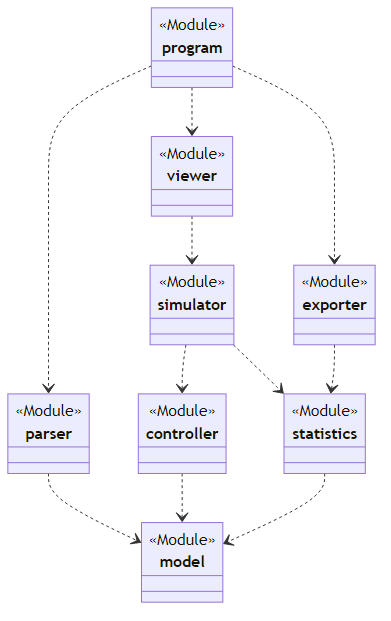
\includegraphics[scale=0.4]{../../diagrams/architecture-v2.png}
    \caption{Software architecture}
    \label{fig:software-architecture}
\end{figure}

In the following, we discuss each module in more detail including their responsibilities and interactions.

\subsection{Module \texttt{model}}
\label{sec:data-model}

The \texttt{model} module provides the core data structures for modeling static system configurations and representing dynamic system states.
Figure~\ref{fig:data-model} shows the respective classes, their attributes, and their relationships.

\begin{figure}[h!]
    \centering
    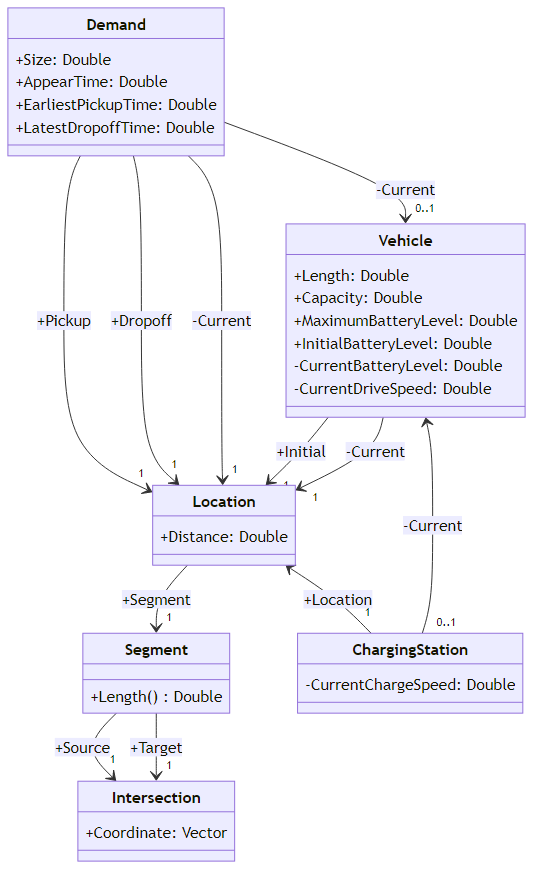
\includegraphics[scale=0.4]{../../diagrams/model/classes-v0.2.png}
    \caption{Data model}
    \label{fig:data-model}
\end{figure}

The \texttt{Intersection} class represents intersections of the driving infrastructure.
Each intersection stores its coordinate in three-dimensional space.
Note that we use Cartesian coordinates for simplicity.

The \texttt{Segment} class represents road segments of the driving infrastructure.
Each segment points to its source and its target intersection.
Furthermore, each segment provides a method for computing its length.
Note that we use the Euclidean distance between source and target intersection here.

The \texttt{Location} class represents specific points on the segments of the driving infrastructure.
Each location points to the corresponding segment of the driving infrastructure.
Furthermore, each location stores a distance on this segment.
The distance is measured in Eclidean units of the Cartesian space.

The \texttt{ChargingStation} class represents the charging infrastructure.
Each charging station stores its location on the driving infrastructure.
Futhermore, each charging station provides its current charging speed.
Note that the simulator computes the current charging speed dynamically.

The \texttt{Vehicle} class \textcolor{red}{TODO}

The \texttt{Demand} class \textcolor{red}{TODO}

\subsection{Module \texttt{controller}}
\label{sec:controller-interface}

%For evaluation of defined system designs, the approach offers an controller interface for defining control strategies. 

\textcolor{red}{TODO}

\begin{figure}[h!]
    \centering
    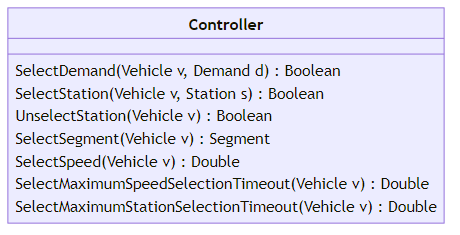
\includegraphics[scale=0.4]{../../diagrams/controller/classes-minimal.png}
    \caption{Controller interface}
    \label{fig:controller-interface}
\end{figure}

For evaluation pruposes, we currently provide five different implementations of the controller interface:
A manual controller (see Section~\ref{sec:controller-manual}), a random controller (see Section~\ref{sec:controller-random}), a greedy controller (see Section~\ref{sec:controller-greedy}), a smart controller (see Section~\ref{sec:controller-smart}), and a switchable controller (see Section~\ref{sec:controller-switch}).

\subsubsection{Manual controller}
\label{sec:controller-manual}

\textcolor{red}{TODO}

\begin{figure}[h!]
    \centering
    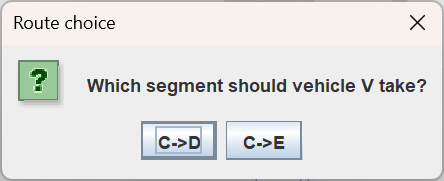
\includegraphics[scale=0.4]{../../screenshots/manual-controller-route.png}
    \caption{Route choice}
    \label{fig:manual-controller-route}
\end{figure}

\textcolor{red}{TODO}

\begin{figure}[h!]
    \centering
    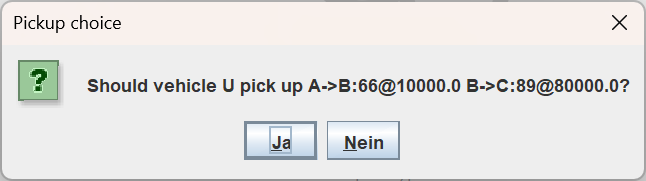
\includegraphics[scale=0.4]{../../screenshots/manual-controller-demand.png}
    \caption{Pickup choice}
    \label{fig:manual-controller-demand}
\end{figure}

\textcolor{red}{TODO}

\begin{figure}[h!]
    \centering
    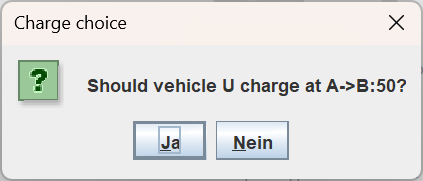
\includegraphics[scale=0.4]{../../screenshots/manual-controller-charge.png}
    \caption{Charge choice}
    \label{fig:manual-controller-charge}
\end{figure}

\textcolor{red}{TODO}

\subsubsection{Random controller}
\label{sec:controller-random}

\textcolor{red}{TODO}

\subsubsection{Greedy controller}
\label{sec:controller-greedy}

\textcolor{red}{TODO}

\subsubsection{Smart controller}
\label{sec:controller-smart}

\textcolor{red}{TODO}

\subsubsection{Switchable controller}
\label{sec:controller-switch}

\textcolor{red}{TODO}

\subsection{Module \texttt{statistics}}
\label{sec:statistics-interface}

\textcolor{red}{TODO}

\begin{figure}[h!]
    \centering
    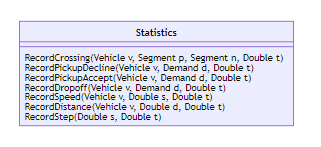
\includegraphics[scale=0.4]{../../diagrams/statistics/classes.png}
    \caption{Statistics interface}
    \label{fig:statistics-interface}
\end{figure}

\textcolor{red}{TODO}

\subsection{Module \texttt{parser}}

\textcolor{red}{TODO}

\subsection{Module \texttt{simulator}}

\textcolor{red}{TODO}

\subsection{Module \texttt{exporter}}

\textcolor{red}{TODO}

\subsection{Module \texttt{viewer}}
\label{sec:gui}

\textcolor{red}{TODO}

%\begin{figure*}[tbp]
%    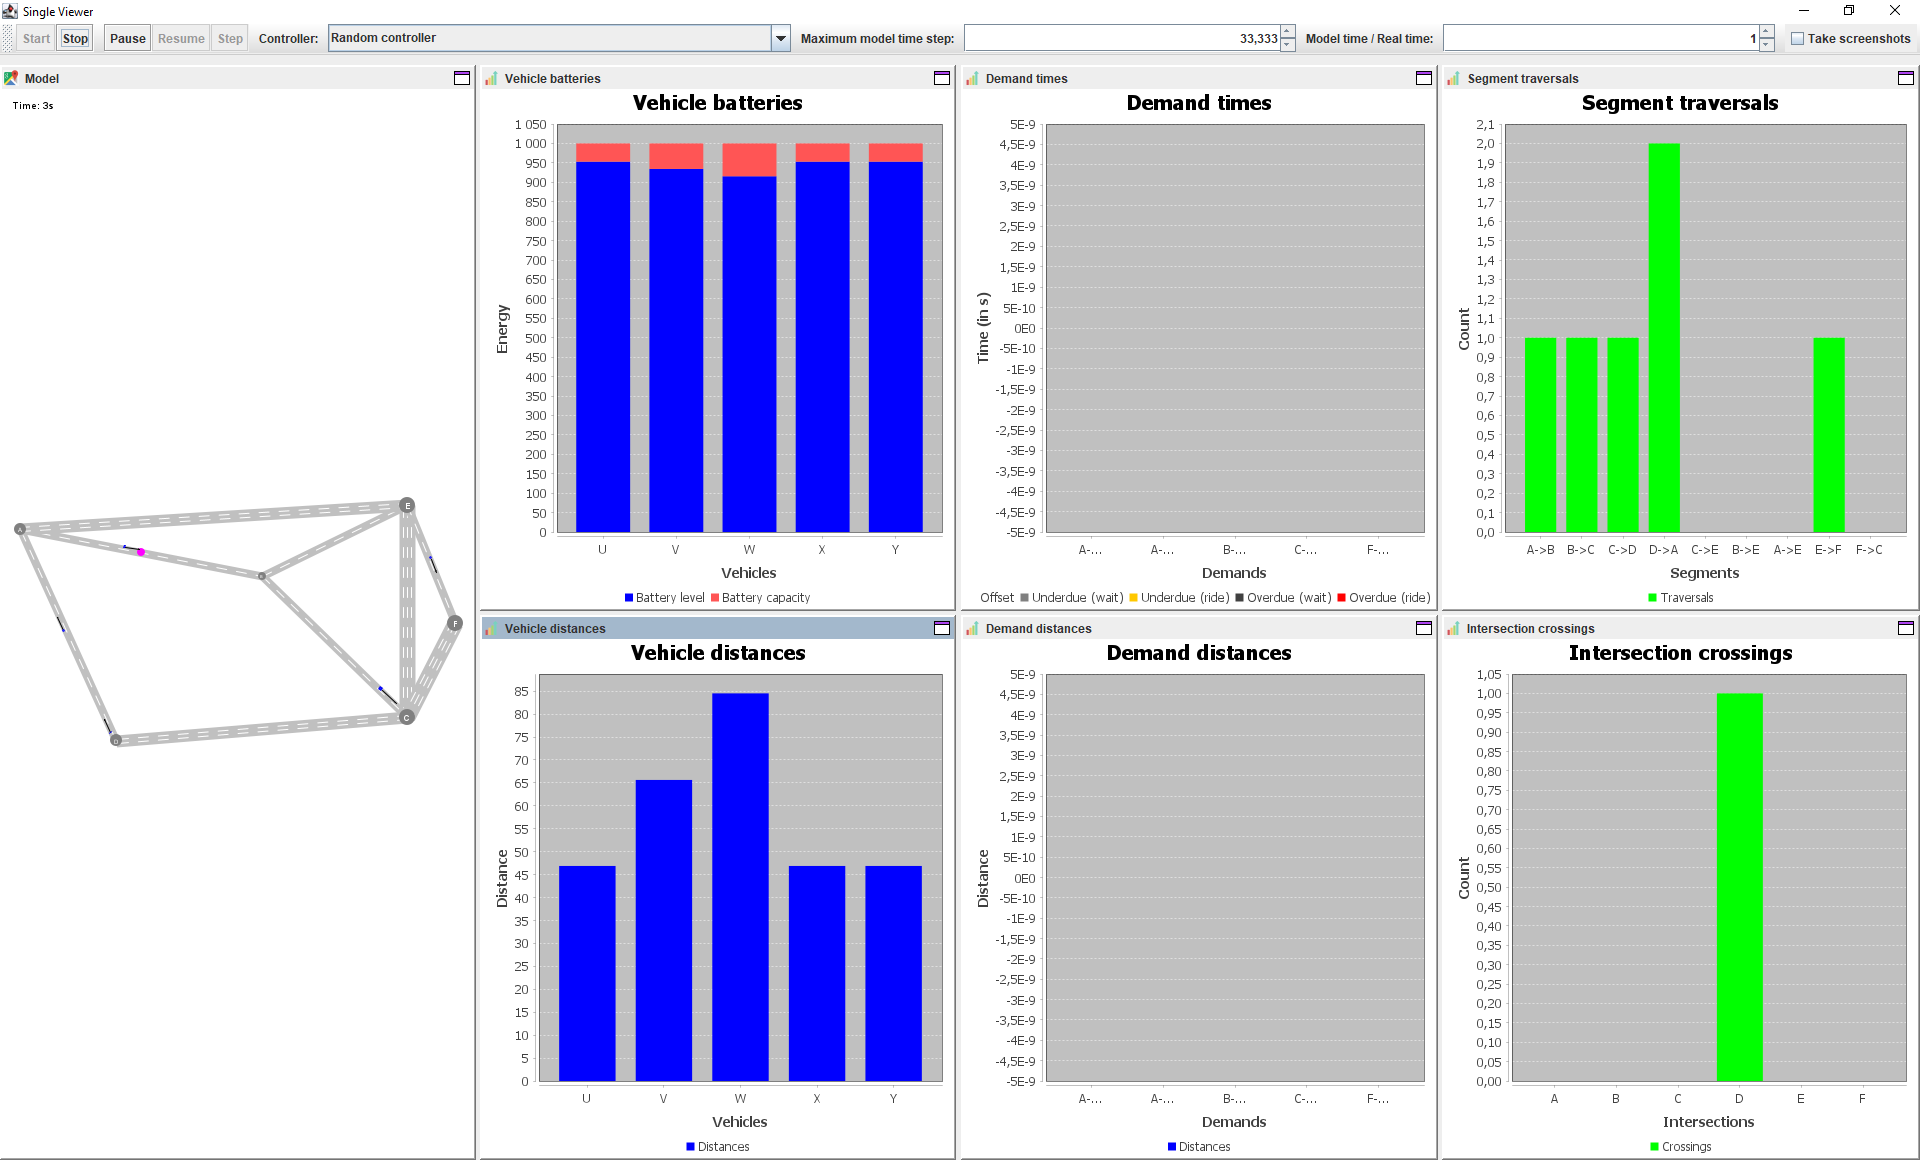
\includegraphics[width=\textwidth]{../../screenshots/basic-simulation.png}
%    \caption{Graphical user interface}
%    \label{fig:gui}
%\end{figure*}

\subsubsection{Map}

\textcolor{red}{TODO}

\subsubsection{Vehicle charts}

\textcolor{red}{TODO}

\paragraph{Vehicle battery chart}

\textcolor{red}{TODO}

\paragraph{Vehicle distance chart}

\textcolor{red}{TODO}

\subsubsection{Demand charts}

\textcolor{red}{TODO}

\paragraph{Demand time chart}

\textcolor{red}{TODO}

\paragraph{Demand distance chart}

\textcolor{red}{TODO}

\subsubsection{Infrastructure charts}

\textcolor{red}{TODO}

\paragraph{Intersection chart}

\textcolor{red}{TODO}

\paragraph{Segment chart}

\textcolor{red}{TODO}

\paragraph{Station chart}

\textcolor{red}{TODO}

\subsection{Module \texttt{program}}
\label{sec:application}

\textcolor{red}{TODO}

\subsubsection{Controller comparison}
\label{sec:controller-comparison}

\textcolor{red}{TODO}

\begin{figure*}[tbp]
    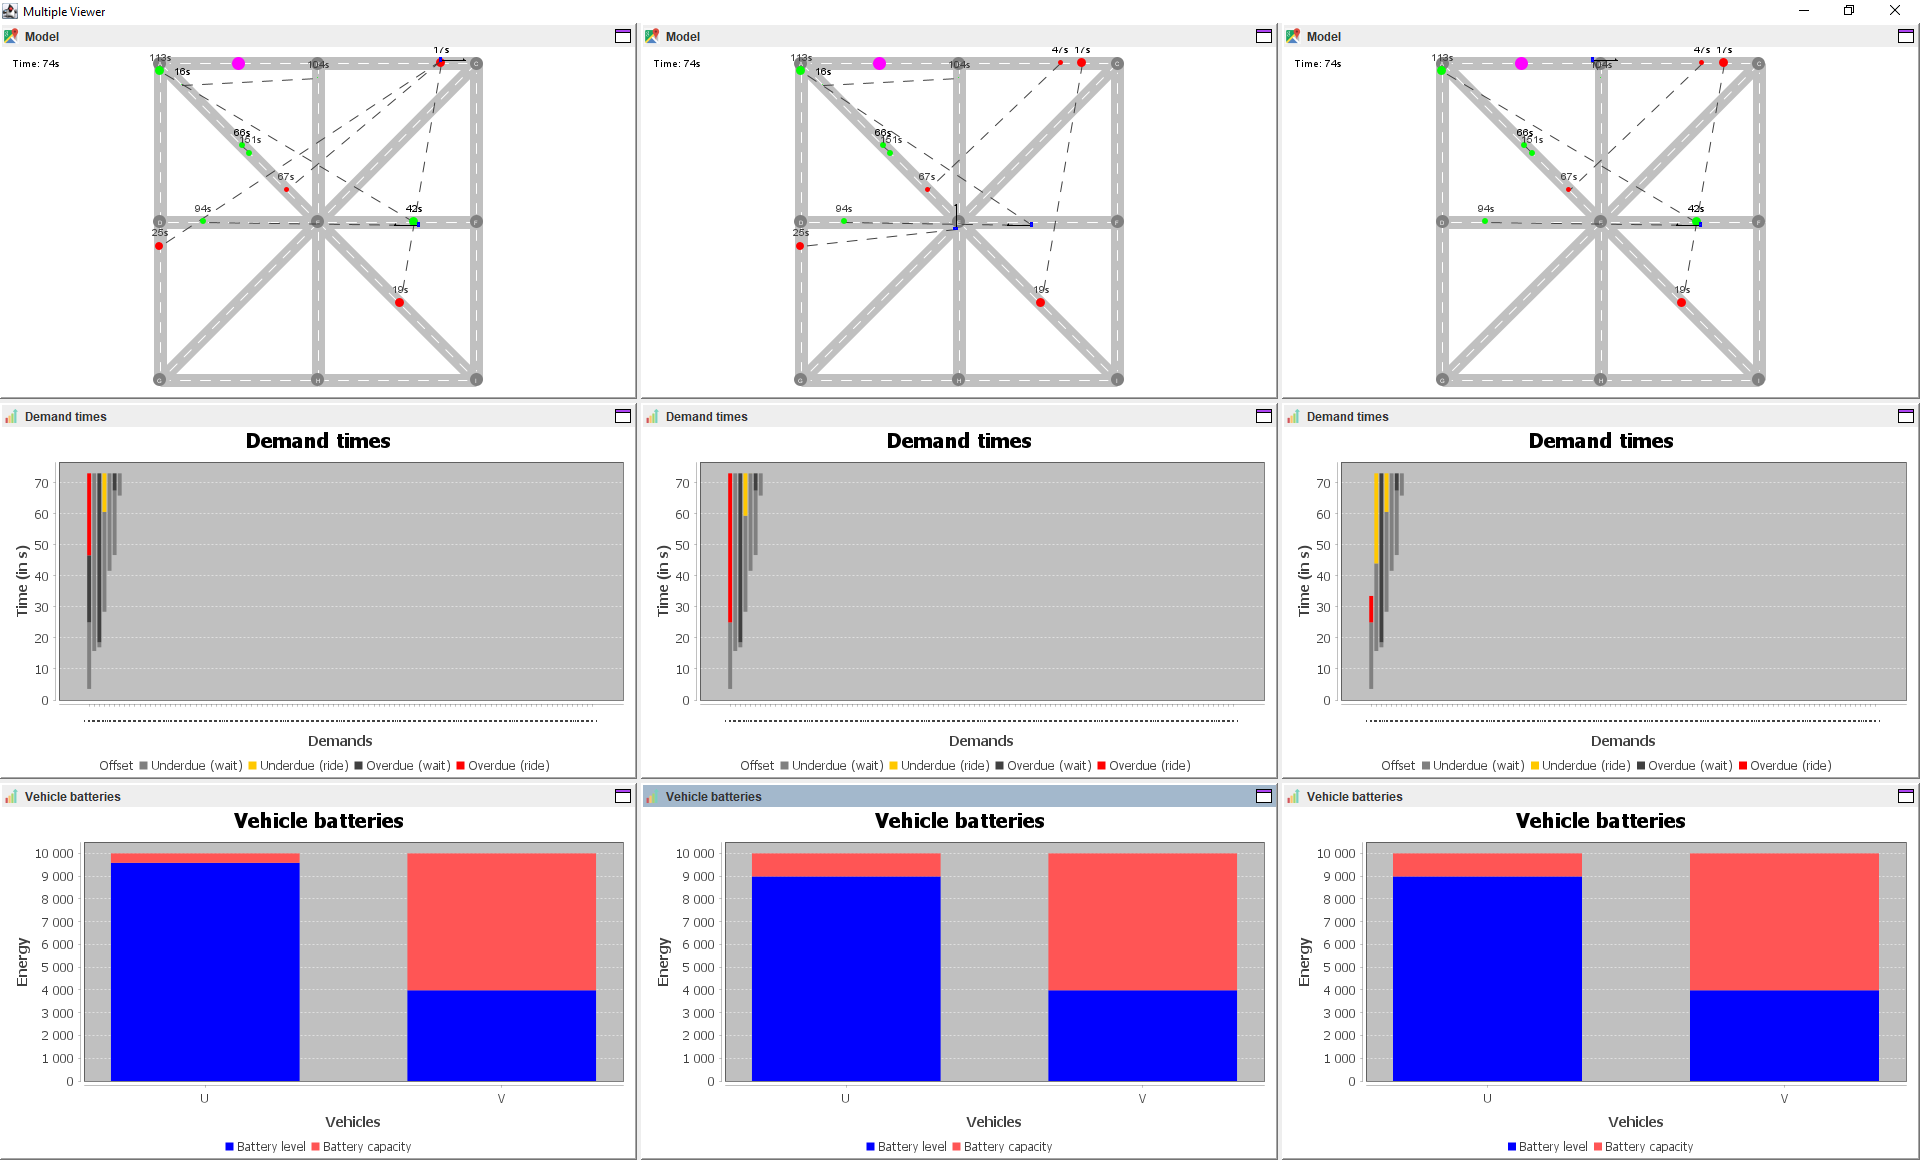
\includegraphics[width=\textwidth]{../../screenshots/controller-comparison.png}
    \caption{Controller comparison}
    \label{fig:controller-comparison}
\end{figure*}

\textcolor{red}{TODO}

\subsubsection{Infrastructure comparison}
\label{sec:infrastructure-comparison}

\textcolor{red}{TODO}

\begin{figure*}[tbp]
    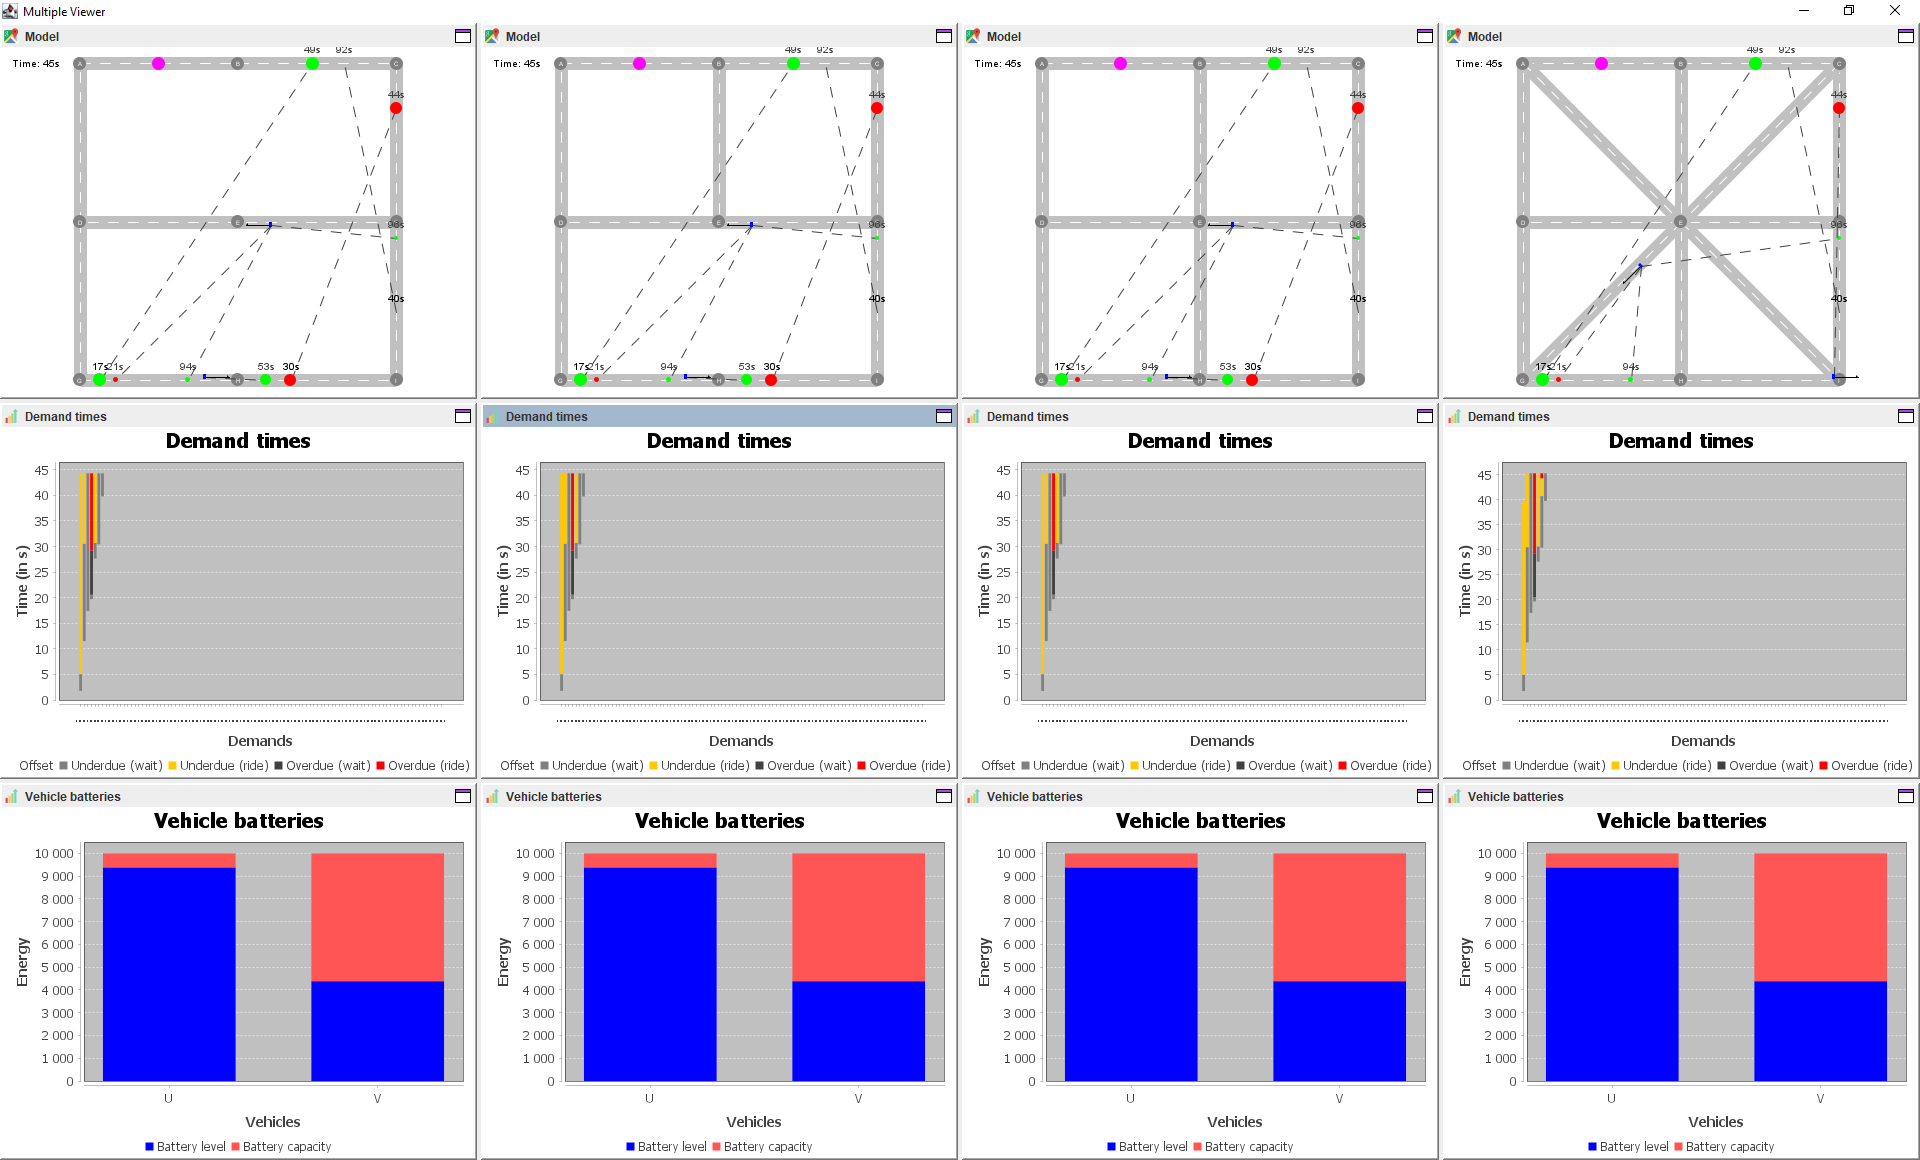
\includegraphics[width=\textwidth]{../../screenshots/infrastructure-comparison.png}
    \caption{Infrastructure comparison}
    \label{fig:infratructure-comparison}
\end{figure*}

\textcolor{red}{TODO}

\section{Conclusion}
\label{sec:conclusion}

\textcolor{red}{TODO}

\bibliographystyle{plain}
\bibliography{main}

\end{document}
